\let\negmedspace\undefined
\let\negthickspace\undefined
\documentclass[journal]{IEEEtran}
\usepackage[a5paper, margin=10mm, onecolumn]{geometry}
%\usepackage{lmodern} % Ensure lmodern is loaded for pdflatex
\usepackage{tfrupee} % Include tfrupee package

\setlength{\headheight}{1cm} % Set the height of the header box
\setlength{\headsep}{0mm}     % Set the distance between the header box and the top of the text
\usepackage{multicol}
\usepackage{gvv-book}
\usepackage{gvv}
\usepackage{cite}
\usepackage{amsmath,amssymb,amsfonts,amsthm}
\usepackage{algorithmic}
\usepackage{graphicx}
\usepackage{textcomp}
\usepackage{xcolor}
\usepackage{txfonts}
\usepackage{listings}
\usepackage{enumitem}
\usepackage{mathtools}
\usepackage{gensymb}
\usepackage{comment}
\usepackage[breaklinks=true]{hyperref}
\usepackage{tkz-euclide} 
\usepackage{pgfplots}
\pgfplotsset{compat=1.18}
\usepackage{listings}
% \usepackage{gvv}                                        
\def\inputGnumericTable{}                                 
\usepackage[latin1]{inputenc}                                
\usepackage{color}                                            
\usepackage{array}                                            
\usepackage{longtable}                                       
\usepackage{calc}                                             
\usepackage{multirow}                                         
\usepackage{hhline}                                           
\usepackage{ifthen}                                           
\usepackage{lscape}
\usepackage{tikz}
% Marks the beginning of the document
\begin{document}
\bibliographystyle{IEEEtran}
\vspace{3cm}

\title{Solving differential equation\\NCERT-9.5.4}
\author{EE24BTECH11056 - S.Kavya Anvitha}
\maketitle
%\newpage
\bigskip

\renewcommand{\thefigure}{\theenumi}
\renewcommand{\thetable}{\theenumi}
\textbf{simuluation method}

\text{Given:}
\begin{align}
\frac{dy}{dx} + \sec(x) \cdot y &= \tan(x)
\end{align}

\text{Rewriting:}
\begin{align}
\frac{dy}{dx} &= \tan(x) - y \cdot \sec(x)
\end{align}

\text{Using the definition of derivative:}
\begin{align}
\lim_{h \to 0} \frac{y\brak{x+h} - y\brak{x}}{h} &= \tan(x) - y \cdot \sec(x)
\end{align}

\text{Approximating for small $h$:}
\begin{align}
\frac{y_{n+1} - y_n}{h} &\approx \tan(x) - y \cdot \sec(x)
\end{align}

\text{Reorganizing:}
\begin{align}
y_{n+1} - y_n &= h \cdot \frac{dy}{dx}
\end{align}

\text{Therefore:}
\begin{align}
y_{n+1} &= y_n + h \cdot \frac{dy}{dx}
\end{align}
\begin{align}
y_{n+1} &= y_n + h \cdot \brak{\tan(x_n) - y_n \cdot \sec(x_n)}
\end{align}
By initializing the values of x and y and iterating the process several times 
and plotting them gives the curve for solution of the differential equation\\

\textbf{Theoretical solution:}\\
Consider the differential equation:

\begin{align}
\frac{dy}{dx} + \sec(x)y = \tan(x)
\end{align}

where $0 \leq x < \frac{\pi}{2}$.

This is a first-order linear differential equation of the form:

\begin{align}
\frac{dy}{dx} + P(x)y = Q(x)
\end{align}

where $P(x) = \sec(x)$ and $Q(x) = \tan(x)$.

The integrating factor (IF) is given by:

\begin{align}
I(x) &= e^{\int P(x) \, dx} = e^{\int \sec (x), dx}.
\end{align}

The integral of $\sec(x)$ is:

\begin{align}
\int \sec(x) \, dx = \ln \abs {\sec(x) + \tan(x)}.
\end{align}

Thus, the integrating factor becomes:

\begin{align}
I(x) = e^{\ln\abs{\sec(x) + \tan(x)}} = \abs{\sec(x) + \tan(x)}.
\end{align}

Applying the integrating factor to the differential equation:

\begin{align}
\frac{d}{dx}\brak{ y \cdot \abs{\sec(x) + \tan(x)}} &= \tan(x) \abs{\sec(x) + \tan(x)}.
\end{align}

Integrate both sides:

\begin{align}
y \cdot \abs{\sec(x) + \tan(x)} &= \int \tan(x) \abs{\sec(x) + \tan(x)} \, dx.
\end{align}

Observe that the derivative of $\sec(x) + \tan(x)$ is $\sec(x)\tan(x) + \sec^2(x)$, so the integral simplifies to:

\begin{align}
y \cdot \abs{\sec(x) + \tan(x)} &= \abs{\sec(x) + \tan(x)} + C.
\end{align}

Therefore, the general solution is:

\begin{align}
y = 1 + \frac{C}{\abs{\sec(x) + \tan(x)}}
\end{align}

where $C$ is the constant of integration.

\begin{figure}[h!]
   \centering
   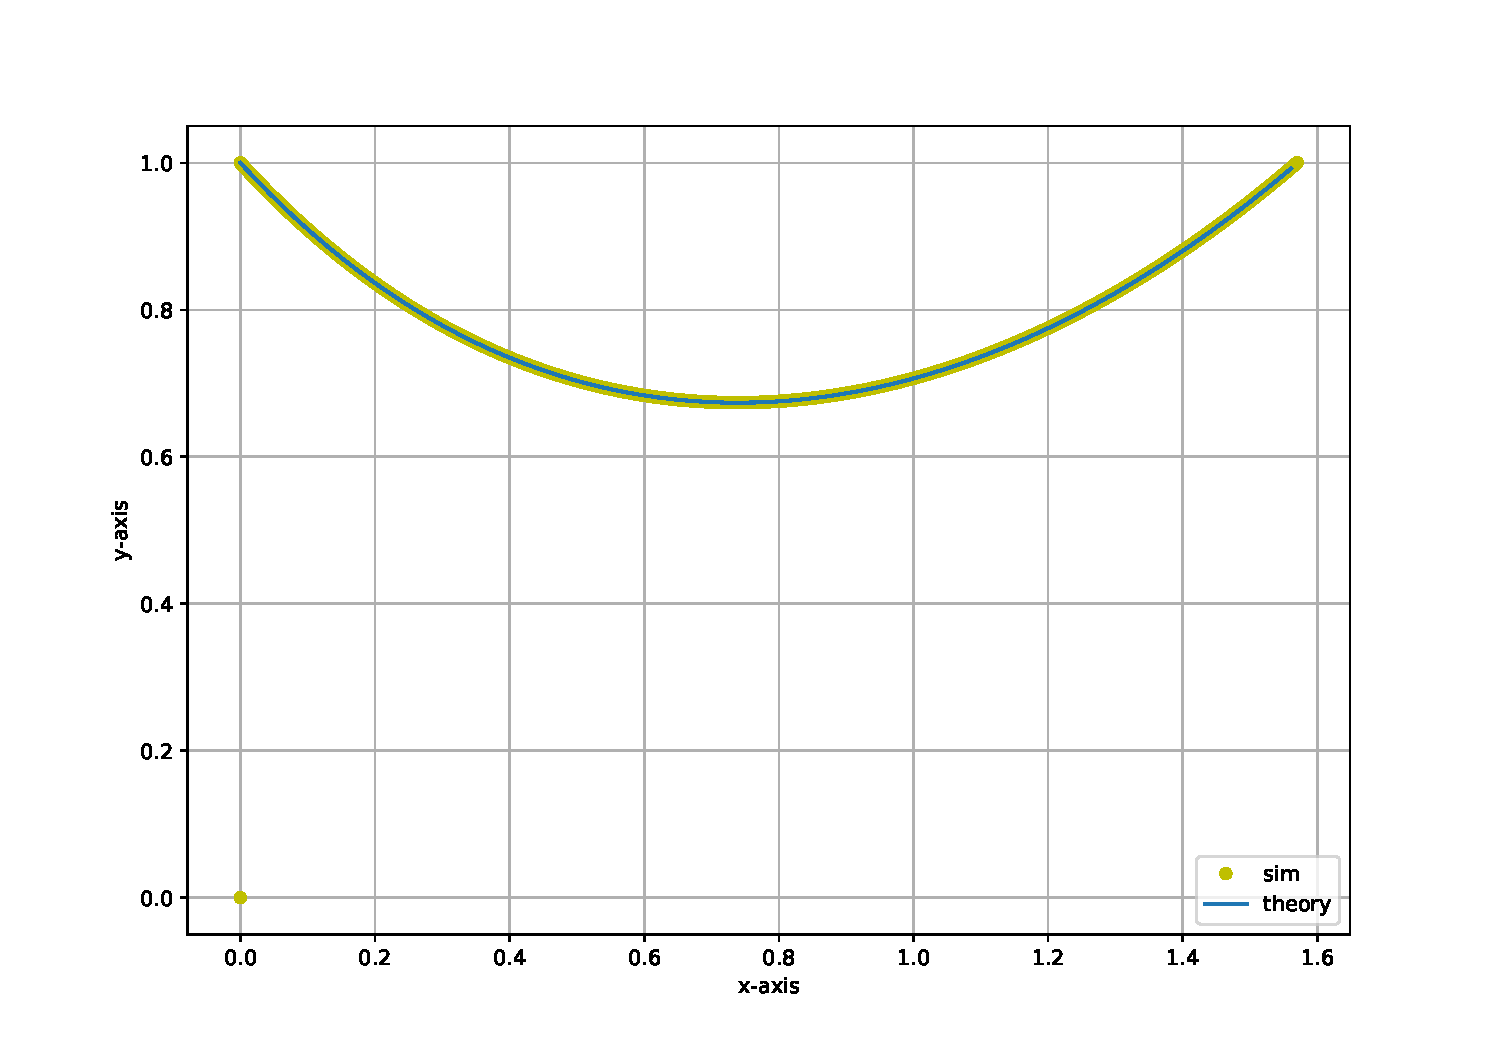
\includegraphics[width=0.7\columnwidth]{figs/combined_plot.pdf}
\end{figure}


\end{document}

